\documentclass[11pt,twoside]{article}
\usepackage{fullpage}
\usepackage{epsf}
\usepackage{fancyhdr}
\usepackage{graphics}
\usepackage{graphicx}
\usepackage{psfrag}
\usepackage{microtype}
\usepackage{subfigure}
\usepackage{algorithmic}
\usepackage[dvipsnames]{color,xcolor}
\usepackage[linesnumbered,ruled]{algorithm2e}% http://ctan.org/pkg/algorithm2e
\DontPrintSemicolon
\usepackage{color}
\usepackage{tabularx}
\usepackage{amsthm}
\usepackage{amsfonts}
\usepackage{amsmath}
\usepackage{amssymb,bbm}
\usepackage{stackengine}
\usepackage{footnote}
\makesavenoteenv{tabular}
\makesavenoteenv{table}
\usepackage{natbib}
\usepackage{caption}
\usepackage{subcaption}
\usepackage{url}% for url's in bib
% for theorem hyperlink colors
\usepackage[colorlinks,linkcolor=OliveGreen,citecolor=OliveGreen, backref=true]{hyperref}
% \renewcommand*{\backref}[1]{\ifx#1\relax \else Page #1 \fi}
\renewcommand*{\backrefalt}[4]{%
    \ifcase #1 \footnotesize{(Not cited.)}%
    \or        \footnotesize{(Cited on page~#2.)}%
    \else      \footnotesize{(Cited on pages~#2.)}%
    \fi}

% for nice fractions
\usepackage{nicefrac}
\usepackage{comment}

% for adjust width
\usepackage{chngpage}

 \usepackage{tabularx}%

% to label enumerate
\usepackage{enumitem}
% Top and bottom rules for tables
\usepackage{booktabs}
% for captions
\usepackage{caption}

\usepackage{bm,bbm}
% for mathmakebox
\usepackage{mathtools}

\newcommand{\strongconvex}{\mu}
%\newcommand{\smooth}{\smooth}
%\newcommand{\smoothprior}{L_2}
\newcommand{\subgaussian}{\sigma}
%\newcommand{\discretizedFn}{\discretized{F}_n}
%
\usepackage{amsthm}

\theoremstyle{definition}
\newtheorem{definition}{Definition}[section]
\newtheorem{assumption}{Assumption}
\newtheorem{theorem}{Theorem}[section]
\newtheorem{corollary}{Corollary}[theorem]
\newtheorem{lemma}[theorem]{Lemma}
%%%%%%%%%%%%%%%%%%%%%%%%%%%%%%%%%%%%%%%%%%%%%%%%%
\setlength{\textwidth}{\paperwidth}
\addtolength{\textwidth}{-6cm}
\setlength{\textheight}{\paperheight}
\addtolength{\textheight}{-4cm}
\addtolength{\textheight}{-1.1\headheight}
\addtolength{\textheight}{-\headsep}
\addtolength{\textheight}{-\footskip}
\setlength{\oddsidemargin}{0.5cm}
\setlength{\evensidemargin}{0.5cm}
%%%%%%%%%%%%%%%%%%%%%%%%%%%%%%%%%%%%%%%%%%%%%%%%%
%\newtheorem{lemma}{Lemma}
%\newtheorem{theorem}{Theorem}
%\newtheorem{proposition}{Proposition}
%\newtheorem{definition}{Definition}
%\newtheorem{corollary}{Corollary}%opening
%\newtheorem{assumption}{Assumption}
%\newtheorem{conjecture}{Conjecture}
\newenvironment{assumptionprime}[1]
  {\renewcommand{\theassumption}{\ref{#1}$'$}%
   \addtocounter{assumption}{-1}%
   \begin{assumption}}
  {\end{assumption}}
\newcommand{\cheeger}{\mathfrak{h}}

\newcommand{\Wass}{\ensuremath{\mathcal{W}}}
%
%\newcommand{\real}{\ensuremath{\mathbb{R}}}

%%% New version of \caption puts things in smaller type, single-spaced 
%%% and indents them to set them off more from the text.h
\makeatletter
\long\def\@makecaption#1#2{
        \vskip 0.8ex
        \setbox\@tempboxa\hbox{\small {\bf #1:} #2}
        \parindent 1.5em  %% How can we use the global value of this???
        \dimen0=\hsize
        \advance\dimen0 by -3em
        \ifdim \wd\@tempboxa >\dimen0
                \hbox to \hsize{
                        \parindent 0em
                        \hfil 
                        \parbox{\dimen0}{\def\baselinestretch{0.96}\small
                                {\bf #1.} #2
                                %%\unhbox\@tempboxa
                                } 
                        \hfil}
        \else \hbox to \hsize{\hfil \box\@tempboxa \hfil}
        \fi
        }
\makeatother
\newcommand{\tr}{\text{tr}}
\newcommand{\Prb}{\mathbb{P}}
\newcommand{\E}{\mathbb{E}}
\newcommand{\R}{\mathbb{R}}
\newcommand{\bfx}{\mathbf{x}}
\newcommand{\bX}{\mathbf{X}}
\newcommand{\KL}{\text{KL}}


\usepackage{algorithm}
\usepackage{algpseudocode}
\usepackage[many]{tcolorbox}
\newtcolorbox{boxK}{
    sharpish corners, % better drop shadow
    boxrule = 0pt,
    toprule = 4.5pt, % top rule weight
    enhanced,
    fuzzy shadow = {0pt}{-2pt}{-0.5pt}{0.5pt}{black!35} % {xshift}{yshift}{offset}{step}{options} 
}
\newtcolorbox{boxF}{
    colback = sub,
    enhanced,
    boxrule = 1.5pt, 
    colframe = white, % making the base for dash line
    borderline = {1.5pt}{0pt}{main, dashed} % add "dashed" for dashed line
}


\title{\textsc{Langevin Monte Carlo without log-concavity}}
\author{Leello Dadi}
\date{}


\begin{document}

\maketitle

\begin{abstract}
    Langevin Monte Carlo (LMC) is a Markov Chain Monte Carlo sampling method that generate samples by adding gradient information to Gaussian noise. Since it queries only local information, we might expect it to have all the limitations of local methods like Gradient Descent. The presence of noise, however, makes LMC capable of provably sampling from a large class of distributions for which global information cannot be inferred from local queries. 
    
    This statement was proved by Vempala and Wibisono in \cite{vempala_rapid_2019} under two mild assumptions. This will be the starting point of our report. We will then see that, although their work shows the region of tractability for LMC extends beyond strong log-concavity, there is a potential exponential blow-up of constants in the convergence bound that ensures that the computational hardness of non-convexity is never violated. Tzen et al's trajectory-wise analysis of LMC \cite{tzen_local_2018} will shed some light on the causes of this exponential blow-up of convergence time. With this understanding, we will naturally ask whether or not this blow-up occurs when trying to sample from real world distributions. By discussing the success of Song and Ermon's work \cite{song_generative_2019} using LMC to generate natural images, we will finish by arguing that the real world may well be within the tractable region.
\end{abstract}

\section{Introduction}

In keeping with the tradition of secretive Monte Carlo research initiated by Ulam and Von Neuman \cite{eckhardt_stan_nodate}, we will consider in this report the problem of sampling from a probability distribution $\pi$ while keeping secret our motivations for doing so. 

The considered distribution $\pi$, our target measure, is a probability measure over $\R^d$ that admits a density $p_\pi$ that can be expressed as
\[
p_\pi(x) = \frac{\exp{\left(-f(x)\right)}}{Z},
\]
where $f: \R^d \mapsto \R$ is a continuously differentiable function, referred to as the \textit{potential}, and $Z \in \R$ is a normalization constant. We assume that we can query $f$ and $\nabla f$ at any point $x \in \R^d$, but $Z$ will remain unknown.

Our goal is to generate samples approximately distributed according to $\pi$. One approach for doing so is to initialize a random walk at some point $\bX_0 \in \R^d$ and make Gaussian steps exploring the space hoping to land in the typical regions of $\pi$ \cite{sherlock_random_2010}. Before committing to a step, we can check if the walk is leading us towards a higher probability regions by querying $f$ then decide to accept or reject this step. Eventually our random walk will output samples from $\pi$ at the risk of having to reject many steps. 

Here, however, since we have access to the gradients, we can inform our random walk by using this first-order information: the gradient can guide us towards high probability regions. This is the idea of Langevin Monte Carlo (LMC). The algorithm consists of generating the following Markov Chain 
\begin{equation}
\bX_{k+1} = \bX_k - \eta \nabla f(\bX_k) + \sqrt{2\eta}\mathbf{Z}_{k+1},
\label{eq:LMC}
\tag{LMC}
\end{equation}
where $\eta > 0$ is referred to as the step-size and $(\mathbf{Z}_k)_k$ is an sequence of independent identically distributed $\mathcal{N}(0, 1)$ variables.

LMC is a gradient augmented random walk and using it sample was first suggested in the chemical physics literature \cite{rossky_brownian_1978}. The asymptotic convergence of the scheme for a fixed step-size was discussed in \cite{roberts_exponential_1996} and the authors argued for the necessity of an Metropolis accept/reject step to ensure that the iterates would eventually sample from $\pi$.

Indeed, without such a step, the distributions of the iterates $(\bX_k)_{k\in \mathbb{N}}$ tend to a biased limit $\pi_\eta$, that is in most cases different from $\pi$. Dalalyan \cite{dalalyan_theoretical_2016}, through a non asymptotic analysis, offered a possible way of side stepping this need for a Metropolis filter. He showed that given a precision $\epsilon$, it was possible to pick $\eta$ small enough, then run the \eqref{eq:LMC} chain for long enough to generate samples that were $\epsilon$ close $\pi$.

The non-asymptotic convergence guarantees were first derived in the strongly-log-concave case \cite{dalalyan_theoretical_2016}, i.e when $f$ is strongly convex. In this report our focus will be on guarantees of convergence that do not require strong-convexity or even convexity of $f$. This is of particular interest because \eqref{eq:LMC} only sees $f$ through local queries of the gradient and one may believe some form of convexity, or conditions on stationary points, would be necessary to obtain strong guarantees. The presence of noise seems to dispense with the need for such strong conditions when sampling is the goal.

We will see that it is possible to establish convergence of \eqref{eq:LMC} under two mild assumptions that, in effect, only put restrictions on the tails of $f$. The proof we will study is Vempala and Wibisono's in \cite{vempala_rapid_2019} where they show convergence of the iterates as measured by the KL divergence from $\pi$ (Section \ref{sec:vemp}).

The convergence bound will, at first sight, appear to always be polynomial in dimension. But a closer inspection, informed by the work of Tzen, Liang and Raginsky \cite{tzen_local_2018}, will reveal that the convergence can be extremely slow, and in fact be exponential in dimension. The divide between the tractable realm of polynomial convergence and the intractable is captured by a single constant appearing in the bound : the log-Sobolev constant. 

It seems that this log-Sobolev constant is a good measure of benign non-convexity \cite{cheng_sharp_2020, li_escape_2021, pillaud-vivien_statistical_2020}: a sequence involving the sum of a gradient term and a noise term seems to be able to tackle non-convexity as long as the log-Sobolev constant does not have a poor dependence on dimension.

Naturally, we will ask whether or not the real world exhibits this benign non-convexity. Distributions like images, are at the very least multi-modal and therefore cannot be log-concave let alone strongly log-concave. They could however have log-Sobolev constants that have a good polynomial dependence on dimension. Song and Ermon propose a method for applying \eqref{eq:LMC} to real-world distributions. By studying their work, we will discuss whether or not  their results provide sufficient evidence for the claim that the real-world admits well-behaved log-Sobolev constants.

We will conclude by discussing open questions regarding convergence of \eqref{eq:LMC} and reviewing the possible ways in which the tools we understood here to analyze \eqref{eq:LMC} can help us analyze the closely related iterates of Stochastic Gradient Descent, an algorithm in heavy use today, that also mixes gradients with noise, albeit with a different weighing.

\section{Notation and setting}

The distributions considered in this report are measures over $(\R^d, B(\R^d))$, where $B(\R^d)$ denotes the Borel sigma field. The Euclidean norm on $\R^d$ is denoted $\|\cdot\|$. For a probability distribution $\nu$, we write $p_\nu$ for its Lebesgue density. The expectation with respect to $\nu$ is denoted $\E_\nu$. The gradient of a function $f: \R^d \rightarrow \R$ is denoted $\nabla f$, if it is multivariate, the Jacobian is denoted $J_f$. A function is said to be $L$-\textit{smooth} if its gradient is $L$-Lipschitz. We will consider Ito stochastic differential equations of the form 
\[
dX_t =  b(X_t)dt + \sigma dB_t,
\]
where $\sigma > 0$, $(B_t)_{t\in [0, +\infty[}$ is a standard Brownian motion on $\R^d$, and $b: \R^d \mapsto \R^d$ is Lipschitz. For appropriate initializations $X_0$, this equation has a unique solution (Theorem 5.2.1 \cite{oksendal_stochastic_2003}) and for each $t\in [0, +\infty[$, the law of $X_t$ admits a density denoted $p_t$ with respect to the Lebesgue measure, moreover, $t \mapsto p_t$ is continuously differentiable (Thm 4.1 \cite{pavliotis_fokkerplanck_2014}). 

The $\KL$ divergence from $\pi$ of a measure $\nu$ and the relative Fisher information I of $\nu$ with respect to $\pi$ are defined as
\[
\KL(\nu || \pi) = \int_{\R^d} p_\nu(x)\log\frac{p_\nu(x)}{p_\pi(x)}dx \quad \text{and} \quad I(\nu || \pi) = \int_{\R^d} p_\nu(x)\left\|\nabla \log\frac{p_\nu(x)}{p_\pi(x)}\right\|^2dx.
\]

\section{Convergence under isoperimetry and smoothness}
\label{sec:vemp}
We begin our study with the proof that the distribution of iterates $(\bX_k)_k$, for an appropriate fixed step-size $\eta$, will indeed approach the target distribution $\pi$. 

As Vempala and Wibisono's show, this convergence will hold even without convexity of the potential $f$. A convergence analysis for two divergence measures is provided in their paper\cite{vempala_rapid_2019}, the $\KL$ and the Renyi divergence. Our focus will be on the $\KL$ divergence as it the more complete contribution of the paper.

The main result of \cite{vempala_rapid_2019} is a bound on the decrease of $\KL$ divergence at each single step of \eqref{eq:LMC}, when going from $\bX_k$ to $\bX_{k+1}$. The convergence of the whole sequence is then obtained by induction. Two assumptions are needed for this result. The first is smoothness of the target potential. The second is a functional inequality called the log-Sobolev inequality \eqref{eq:LSI}, which we will examine shortly. Using only these two, Vempala and Wibisono prove the following theorem. 


\begin{theorem}
Let $\pi$ be a distribution satisfying the \eqref{eq:LSI} with constant $\alpha > 0$. If the potential is $L$-smooth, we have for any $\eta < \frac{\alpha}{4L^2}$, the following decrease at each step:
\[
\KL(\rho_{k+1} || \pi) \leq e^{-\alpha \eta}\KL(\rho_{k} || \pi) + 6\eta^2 d L^2,
\]
where $\rho_k$ denotes the distribution of $\bX_k$.
\label{thm:step}
\end{theorem}

In this section, we will first discuss the \eqref{eq:LSI} assumption to get a better grasp of the scope of the result. We will then discuss the proof of Theorem \ref{thm:step}. After briefly mentioning the Renyi result, we will discuss the implications of the convergence bound.

\subsection{The log-Sobolev inequality}

The main assumptions the authors of \cite{vempala_rapid_2019} is one they refer to as an \textit{isoperimetric} assumption. In particular, they assume that $\pi$ verifies the log-Sobolev inequality. This inequality relates the KL divergence from $\pi$ to the relative Fisher information with respect to $\pi$. It is defined as follows.

\begin{definition}
  There exists $\alpha >0$ such that for any probability measure $\nu$ over $\R^d$ such that $\KL(\nu || \pi) < \infty$, we have
  \begin{equation}
  \KL(\nu || \pi) \leq \frac{1}{2\alpha} I(\nu || \pi).
  \label{eq:LSI}
  \tag{LSI}
  \end{equation}
\end{definition}

The biggest $\alpha$ for which the inequality above holds is called the log-Sobolev constant of $\pi$. This inequality was first introduced by Gross \cite{gross_logarithmic_1975} and we can view it as merely an analytic tool to show sub-gaussian concentration through a line of reasoning called the Herbst argument. 

\begin{boxK}
\paragraph{The Herbst argument} Given a zero mean, real random variable $X$, a concentration inequality is a bound on the tails of the law of $X$. The random variable is said to be sub-gaussian if it verifies the following inequality:
\[
\Prb(|X| > t) \leq C\exp(-\frac{t^2}{c}),
\]
for some absolute constants $C, c > 0$. The Chernoff method, which is a simple application of Markov's inequality to $e^{\lambda X}$ for $\lambda >0$ tells us that to establish such a bound, we only need to control the moment generating function $\lambda \mapsto \E[e^{\lambda X}]$. The \textit{Herbst argument} is a basic sequence of steps showing that the log-Sobolev inequality is enough to upper bound the moment generating function and obtain sub-gaussian tails \cite{boucheron_concentration_2013, ane_sur_2000}.
\end{boxK} 

In other words, assuming the \eqref{eq:LSI} is saying that we have an easy way of showing sub-gaussian tails or, correspondingly, of showing the quadratic growth of $f$. This will be our understanding of \eqref{eq:LSI} : it is a convenient guarantee of sub-gaussian concentration. It is however important to note that \eqref{eq:LSI} is strictly stronger than sub-gaussianity. Here, in \cite{vempala_rapid_2019}, the \eqref{eq:LSI} is referred to with the term \textit{isoperimetric} and this comes from the geometric view of measure concentration which quantifies how much measures concentrate around bodies of a certain volume.

The log-Sobolev assumption has been used in prior publications, namely \cite{dalalyan_theoretical_2014},  \cite{raginsky_non-convex_2017} and \cite{ma_sampling_2019}. In those papers, the \eqref{eq:LSI} is derived from stronger assumptions like strong-log-concavity or dissipativity (see Assumption \ref{ass:dissip}). For the first two, \cite{dalalyan_theoretical_2014} and \cite{raginsky_non-convex_2017}, the stronger assumptions are used again elsewhere in their results, ensuring that Vempala and Wibisono's result cannot be deduced from theirs. The last paper \cite{ma_sampling_2019}, however, does an almost identical analysis albeit with a slightly more complicated proof for essentially the same Lemma (Lemma 12 in \cite{vempala_rapid_2019} and Lemma 5 in \cite{ma_sampling_2019}). A non-exhaustive diagram of the commonly used assumptions in proving convergence of \eqref{eq:LMC} is provided in Figure \ref{fig:diagram}.
\begin{figure}
    \centering
    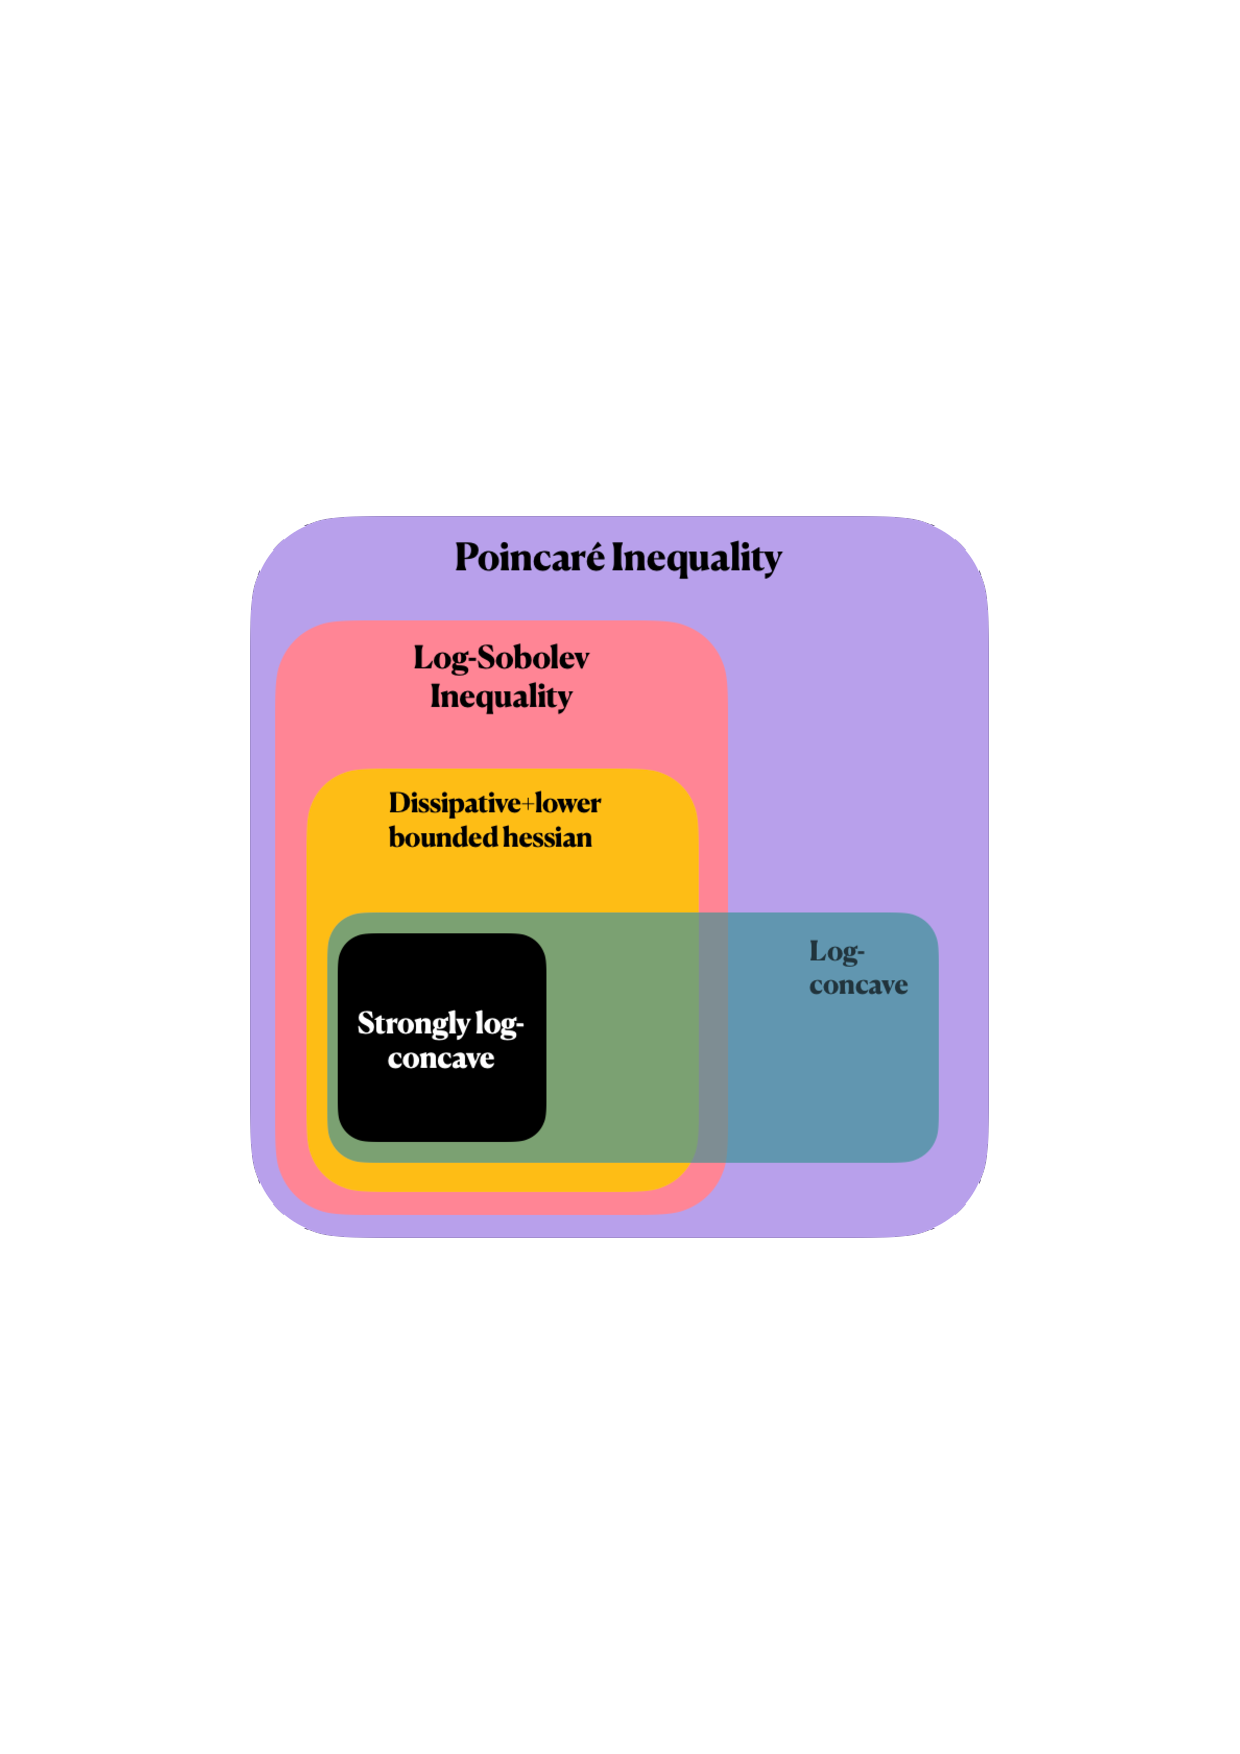
\includegraphics[width=0.5\textwidth]{diagram.pdf}
    \caption{A diagram showing the order between commonly used assumptions.  A proof that strongly-log concave densities are dissipative can be derived from the quadratic lower bound at $0$. Corollary 2.1.(2) of \cite{cattiaux_note_2010} shows that dissipativity and lower bounded hessians imply LSI. The fact that Poincar\'e inequalities  hold for log-concave measures is shown in Corollary 1.9 of \cite{bakry_simple_2008}. The proof that LSI implies Poincar\'e can be found in \cite{bakry_markov_2014}(Proposition 5.1.3).}
    \label{fig:diagram}
\end{figure}

The \eqref{eq:LSI} is a well-behaved inequality in the sense that it is preserved under bounded perturbations of the potential $f$ \cite{ane_sur_2000}. It is also stable through differentiable Lipschitz transformations. This shows that a broad class of distributions verify the \eqref{eq:LSI} and from Figure \ref{fig:diagram} we can see that it is a relatively weak assumptions. Proving convergence without making any stronger additional assumption is therefore a valuable result.

\subsection{A proof through conditional Fokker-Planck}

As mentionned earlier, Vempala and Wibisono prove convergence of \eqref{eq:LMC} by analyzing how the $\KL$ divergence evolves during a single step of \eqref{eq:LMC}. We briefly discuss their proof.

To establish Theorem \ref{thm:step}, the first step is to observe that a single iteration of \eqref{eq:LMC} corresponds to the \textit{exact} solution of the continous-time diffusion

\begin{equation}
    \begin{cases}
        d{X}_t ={\color{MidnightBlue} \nabla f(\bX_k)}dt + \sqrt{2}dB_t \\
        {X}_0 = {\bX_k}
    \end{cases}.
    \label{eq:interp}
\end{equation}

Notice that the {\color{MidnightBlue}drift term} is independent of ${X}_t$ and the exact solution of \eqref{eq:interp} evaluated at time $\eta$ is ${X}_\eta = \bX_{k+1}$. By writing the discrete iterates in this interpolated way, we gain access to the vast toolbox of stochastic differential equations.

Now, our goal is to know how the $KL$ divergence from $\pi$ evolves when going from $\bX_k$ to $\bX_{k+1}$. Using our interpolated process this means we want to know how the continuous object $t \mapsto \KL(p_t || \pi)$ evolves between $t=0$ and $t=\eta$. To do so we compute its time derivative :

\begin{equation}
    \frac{d}{dt}\KL(\rho_t || \pi) = \int_{\mathbb{R}^d} {\color{BrickRed} \frac{\partial \rho_t}{\partial t}}(x)\ln\frac{\rho_t(x)}{\pi(x)}dx.
    \label{eq:kl-deriv}
\end{equation}

From \eqref{eq:kl-deriv}, we see that in order to know the behavior of the $\KL$ divergence, we need to know how the density of $p_t$ of $\hat{X}_t$ evolves, i.e, we need to know ${\color{BrickRed} \frac{\partial \rho_t}{\partial t}}(x)$. 

Luckily for us, since \eqref{eq:interp} is a constant drift diffusion, when conditionned on $\bX_k$, the time derivative $\frac{\partial}{\partial t}{p}_{t|\bX_k}$ of the conditional density is given to us by a standard formula : the Fokker-Planck equation \cite{pavliotis_fokkerplanck_2014}. Once we have the evolution of the conditionned density, we can integrate with respect to $\bX_k$ to determine the evolution of the unconditional density $\frac{\partial}{\partial t}{{p}}_{t}$. This requires a few interchanges between derivatives and expectations.

\begin{boxK}
\paragraph*{On the interchange of derivatives and integrals: } Since we are not integrating over compact domains, the interchange of derivatives and integrals requires justifications. A closely related paper \cite{mou_improved_2019} cares about this interchange and provides lemmas justifying it while \cite{vempala_rapid_2019} does not mention any concerns. A careful read, however, shows that steps resembling the induction argument of \cite{mou_improved_2019} are also done in \cite{vempala_rapid_2019}(Lemma 16, 17) where it is shown that the \eqref{eq:LSI} is preserved when applying the gradient step and adding noise. Since \eqref{eq:LSI} implies sub-gaussian tails, the fast decay required to justify the interchange is obtained as long as the initial distribution verifies the \eqref{eq:LSI} (Theorem 4.1 \cite{pavliotis_fokkerplanck_2014}).
\end{boxK}

\paragraph{} Plugging in \eqref{eq:kl-deriv} the formula for the unconditional density determined through this interchange, we find that
\begin{equation}
    \frac{d}{dt}\KL(\rho_t || \pi) \leq  {\color{Fuchsia}-\frac{3}{4}I(\rho_t || \pi)} + {\color{Bittersweet}\E\left[\| \nabla f(\hat{X}_t) - \nabla f(\bX_k) \|_2^2\right]}.
    \label{eq:bound}
\end{equation}

The {\color{Fuchsia} first} term, ignoring the multiplicative factor, is what we would have obtained if the {\color{MidnightBlue}drift} term in \eqref{eq:kl-deriv} was not frozen in time. The {\color{Bittersweet} second} term is the price we pay for this frozen drift. In other words, it is the price of discretization.

The authors of \cite{vempala_rapid_2019} show that the control of the right hand side of \eqref{eq:bound} can be achieved using only \eqref{eq:LSI} and smoothness.

\subsection{Getting to Gr\"onwall only using LSI and smoothness}

It is clear that the {\color{Fuchsia} first} term in equation \eqref{eq:bound} can immediately be upperbounded using the \eqref{eq:LSI} assumption. An important contribution of this paper is a simple proof showing that the {\color{Bittersweet} second} term can be uniformely bounded for $t \in [0, \eta]$ (Lemma 12, \cite{vempala_rapid_2019}).

The problem boils down to upperbounding the expected squared norm of the gradients of $f$. Vempala and Wibisono show that, as long as $\nabla f$ is Lipschitz smooth, a \textit{transport inequality}, which is an inequality relating a Wassertein distance to the KL divergence, called Talagrand's $T_2$ inequality, is sufficient to control this expected square norm. 

Otto and Villani \cite{otto_generalization_2000} proved that \eqref{eq:LSI} is (strictly) stronger than Talagrand's $T_2$ inequality, consequently, the \eqref{eq:LSI} assumption is sufficient to control the expected squared norms.

With this, the authors are able to derive an inequality roughly of the form
\[
\frac{d}{dt}\KL(\rho_t || \pi) \leq -C\KL(\rho_t || \pi) + D,
\]
where $C, D \geq 0$ are constants. A straightforward application of Gr\"onwall's lemma, which is a common tool to establish exponential decay, yields the result in Theorem \ref{thm:step}.

\subsection{The Renyi Result}

In addition to analyzing the behavior of the $\KL$ divergence along the iterates of \eqref{eq:LMC}, the paper also provides, in a second part, analysis of the evolution of the Renyi divergence.

The Renyi divergence is defined as follows. For a given $q > 0$, the Renyi divergence of order $q$ of $\nu$ from $\pi$, denoted $R_q(\nu || \pi)$, is given by
\[
R_q(\nu || \pi) = \frac{1}{q-1}\log\E_\pi\left[\left( \frac{p_{\nu}(X)}{p_\pi(X)}\right)^q\right].
\]
The Renyi divergence is increasing with respect to $q$, and for $q=1$, we can recover the $\KL$ divergence as a limit. It is therefore a generalisation of $\KL$ for which a generalized version of Pinsker's inequality also holds.

In \cite{vempala_rapid_2019}, it is shown that for a given step size $\eta$, the iterates of \eqref{eq:LMC} converge to the \textit{biased} limit $\pi_\eta$ in Renyi divergence at a fast rate when the biased limit verifies the \eqref{eq:LSI}. A missing result however is how far this biased limit is from the actual target measure $\pi$.

This glaring gap prevents their analysis from being a complete one. They only provide a Gaussian example showing that the assumption that \eqref{eq:LSI} holds for the biased limit and that the distance to the true target is controllable by scaling down $\eta$. For this reason, their analysis is only a first step in proving convergence in Renyi divergence.

Here is how they manage to show their result. The biased limit $\pi_\eta$ is stationnary for the dynamics of \eqref{eq:LMC} : starting from a variable distributed according to $\pi_\eta$, applying a gradient step and then adding gaussian noise returns us back to a variable distributed according to $\pi_\eta$. Observing this, Vempala and Wibisono show that: first, applying a gradient step does not change the Renyi divergence between two distributions and second, adding Gaussian noise, under the \eqref{eq:LSI}, decreases the divergence between distributions by a multiplicative factor.

Putting these two facts together, and exploiting the fact that $\pi_\eta$ is stationnary, \cite{vempala_rapid_2019} show that, at each step of \eqref{eq:LMC}, the Renyi divergence is decreased by a multiplicative factor, thus establishing the fast geometric rate. Without the control of the divergence of this biased limit from the true target, this result remains incomplete.

\subsection{Discussion}

Vempala and Wibisono provide simple and straightforward analysis showing convergence of \eqref{eq:LMC} to the target measure. Indeed a simple induction on Theorem \ref{thm:step}, shows that in order to be $\epsilon$-close in KL divergence to the target measure $\pi$, we can pick $\eta = O(\frac{\alpha \epsilon}{dL^2})$, initialize from an appropriate distribution and run \eqref{eq:LMC} for 
\[
O\left(\frac{L^2d}{\alpha^2\epsilon}\right)
\]
iterations. This convergence time has a polynomial dependence on $d$ only if none of the constants involved are hiding possible dimension dependencies. Since the log-Sobolev inequality encapsulates a very broad class of distributions and is in effect a restriction only on the tails of the potential, it is unreasonable to expect that this convergence time will always be polynomial in dimension. Indeed, any hard non-convex optimization problem can be cast as a sampling problem, as we will see in the next section. And a convergence bound that is always polynomial in dimension  would risk violating the assumptions of computational hardness.

Consequently, some constants in the bound must be hiding possible dimension dependencies and explode exponentially in the dimension for some targets $\pi$. The log-Sobolev constant is the exploding constant. In fact, it is believed that for most generic cases, this constant is exponentially small in dimension \cite{raginsky_non-convex_2017}. In the next section we will give a concrete meaning to the slow convergence time predicted by the bound when LSI constants are very small.

\section{Analyzing the trajectories of LMC}

To better understand how exponentially small LSI constants can affect the dynamics, we turn our attention to the work of Tzen, Liang and Raginsky \cite{tzen_local_2018}. 

The goal of their paper is to describe the behavior of the trajectories of LMC. Here, LMC is viewed as a tool to optimize the potential $f$. This introduces a parameter $\beta$, referred to as the \textit{inverse temperature} in our LMC iteration :
\begin{equation}
\label{eq:betaLMC}
\mathbf{X}_{k+1} = X_k - \eta \nabla f(X_k) + \sqrt{\frac{2\eta}{\beta}}Z_{k+1}
\tag{LMC-$\beta$}
\end{equation}
which is a discretization of the diffusion
\begin{equation}
\label{eq:betadiff}
\tag{LD-$\beta$}
dX_t = -\nabla f(X_t)dt + \sqrt{\frac{2}{\beta}}dB_t.
\end{equation}
The diffusion above has a stationary measure $\pi_\beta$ whose density is proportional to $e^{-\beta f}$. When $\beta \rightarrow \infty$, this stationary measure concentrates around the minimizers of $f$ (Section 3.5, \cite{raginsky_non-convex_2017}). Consequently, by choosing high enough values of $\beta$, we can optimize $f$ using \eqref{eq:betaLMC}.

Tzen et al study the behavior of the iterates of this algorithm around local minimizers of $f$ and they find that with an appropriate choice of $\eta$ and $\beta$, the iterates can be made to stay within the neighborhood of some local minimzer for an arbitrarely long time with high probability.

This indicates that the possibly slow mixing of LMC can be caused by the long times spent around local minimizers.


\subsection{Setting}

In \cite{tzen_local_2018}, the potential $f: \R^d \rightarrow \R$ on which LMC is applied is an empirical risk approximation of a population risk. Indeed, taking the population risk to be of the form
\(
F(x) : = \E_\nu [\ell(x, Z)]
\), where $Z \sim \nu$ is some unknown probability measure over some set $\mathcal{Z}$, we can attempt to optimize $F$ by considering the empirical risk
\begin{equation}
f(x) = \frac{1}{n} \sum_{i=1}^{n}\ell(x, Z_i),
\label{eq:ERM}
\end{equation}
where $Z_1, \dots, Z_n$ are independent, identically distributed samples from $\nu$. The following assumptions are made on the functions $\ell$ which translate to properties of $f$.
\begin{assumption}
  For any $z \in \mathcal{Z}$, the function $x \mapsto \ell(x, z)$ is continuously twice differentiable and there exists $B$ such that $\| \nabla \ell (0, z) \| \leq B$ for all $z \in \mathcal{Z}$.
\end{assumption}
\begin{assumption}
  There exist $L > 0$ and $M> 0$ such that for any $z \in \mathcal{Z}$,
  \[
  \| \nabla \ell(x, z) - \nabla \ell(y, z)\| \leq L \|x - y\| \quad \text{and} \quad \| \nabla^2 \ell(x, z) - \nabla^2 \ell(y, z)\|_2 \leq M \|x - y\|.
  \]
  This implies that $f$ is $L$-Lipschitz gradient and $M$-Lipschitz hessian.
\end{assumption}
\begin{assumption}
  The function $f$ is $(m, b)$-dissipative :
  \[
  \exists m>0, \; b\geq 0, \quad \forall x \in \R^d, \quad \langle x, \nabla f(x) \rangle \geq m \|w\|^2 - b.
  \]
  \label{ass:dissip}
\end{assumption}

We note in passing that these assumptions imply that $f$ verifies the LSI (see Figure \ref{fig:diagram}), but the problem of convergence to stationarity here is not considered here. Rather, Tzen et al focus on proving the following result on time spent around local minima when using \eqref{eq:betaLMC} to optimize \eqref{eq:ERM}.

\subsection{The main result}

We now state the main result of \cite{tzen_local_2018}. First, pick a nondegenerate local minimum $\bar{x}$ of $f$ where $H = \nabla^2f(\bar{x})$ is positive definite and initialize \eqref{eq:betaLMC} within a distance of at most $r > 0$ of $\bar{x}$. 

\begin{quote}
\begin{emph}
For any $\delta \in [0, 1]$, for any small $\epsilon >0$, we set $T_{rec} = \frac{2}{m} \log(\frac{8r}{\epsilon})$. For any escape time $T_{\text{esc}} > T_{\text{rec}}$ of our choice, there exist an $\eta$ small enough, scaling as $O(\frac{1}{T_{\text{esc}}})$, and a $\beta$ big enough, scaling as $O(\log(T_{\text{esc}}))$, such that, for the iterates of \eqref{eq:betaLMC}, we have
\[
\Prb(\text{Escape from $\epsilon$-neighborhood of $w_H$ in } [T_{\text{rec}}, T_{\text{esc}}]) \leq \delta.
\]
\end{emph}
\end{quote}

This result tells us that we can make the iterates of \eqref{eq:betaLMC} stay, with high probability, within the neighborhood of a local minimum for as long as we desire with an appropriate choice of $\eta$ and $\beta$. In other words, there is a choice of $\eta$ and $\beta$ such that \eqref{eq:betaLMC} is trapped close to a local minimum for a long time.

\subsection{A summary of the proof}

We can briefly outline the main ideas underlying the proof. The goal is to control the escape of the discrete iterates from a neighborhood of $\bar{x}$. To do so, we will control the probability that the continuous diffusion \eqref{eq:betadiff} escapes, then we will relate this control to the discretization \eqref{eq:betaLMC}.

\begin{paragraph}{Controlling the escape of diffusion :} The first step is to linearize the gradient around the local minimum $\bar{x}$: we can write $\nabla f(x) = H(x-\bar{x}) - \rho(x - \bar{x})$. This allows us to express the diffusion \eqref{eq:betadiff} as a sum of a well behaved process coming from the linear term and a remainder process coming from the error of the linearization $\rho$. Controlling the escape therefore boils down to controlling the sum of these two processes. At this point, Tzen et al exploit the following seemingly trivial result on the control of a sum.
\begin{lemma}
Let $A$ and $B$ be two real random variables, then the following inclusion of events holds 
\[
\{A + B \geq c \} \subseteq  \{A \geq c_1\} \cup \{ B \geq c_2\}
\]
for \textbf{any} $c_1, c_2$ such that $c_1 + c_2 = c$. 
\end{lemma}

The result above tells us that controlling the sum of two random variables can be achieved by controlling the terms individually with the added benefit of having some freedom to choose the thresholds $c_1$ and $c_2$. In particular if we have some knowledge of $B$ such that we can find a choice of $c_2$ that makes $\Prb(B > c_2) = 0$, \textit{we can shift the entire burden of controlling the sum onto A}.

This is precisely what is done in \cite{tzen_local_2018}. The remainder process, because of the Lipschitzness of the Hessian (Assumption 2), can be upperbounded. Consequently, we can find a choice of threshold that puts the burden of controlling the escape entirely on the well behaved process coming from the linear term. By doing so and by exploiting standard results for the control of the well behaved process, \cite{tzen_local_2018} are able to derive an upper bound on the probability of escape of the diffusion. 
\end{paragraph}

\paragraph{Escape of the discrete process} With the diffusion handled, the goal now is to relate the probability of escape of \eqref{eq:betaLMC} to that \eqref{eq:betadiff}. Previous work, namely the result of Dalalyan \cite{dalalyan_theoretical_2016} as well as \cite{raginsky_non-convex_2017}, has shown that for $\eta$ small enough, the behavior of the discrete process is close to the diffusion \textit{evaluated on a grid}. We would like to simply upper bound the probability of escape of the discrete process with the probability of escape of the diffusion. But, since escape for the discrete process can only be related to escape of the diffusion on a grid, it is \emph{weaker} than controlling the escape on a continuous interval. Indeed, saying that a process does not escape when evaluated on a grid does not exclude the possibility of escape \emph{in between} the grid points. Consequently, a further control of the process in between the grid points is necessary. Adding further conditions on $\eta$ and $\beta$, \cite{tzen_local_2018} are able to do so to prove their result.

\subsection{Is this a compelling theorem ?}

In reading the theorem, we might take issue with the freedom we are given in setting the escape time $T_{\text{esc}}$. The theorem allows us to \emph{choose} how long the process remains trapped. It is less of a theorem on how \eqref{eq:betaLMC} behaves and more of a result on what we can make \eqref{eq:betaLMC} do.

A stronger claim would be one that has $\beta$ chosen independently of $T_{\text{esc}}$. Indeed, we can first choose $\beta$ such that the stationary measure of \eqref{eq:betadiff} concentrates sufficiently around the minimizers of $f$. As shown by \cite{raginsky_non-convex_2017}, $\beta$ only needs to scale polynomially in $d$. And then ask how long the process with take to explore the modes. 

Tzen, Liang and Raginsky allude to such a result in Remark 2 of \cite{tzen_local_2018}. The Eyring-Kramers law they mention relates the mean exit time of a particle following the Langevin diffusion from the neighborhood of a local minimum to the \textit{height of the barrier} it has to cross, i.e the difference in function value between the minimum and the saddle point it has to cross to exit. This exit time was first related to the log-Sobolev constant by \cite{menz_poincare_2014-1}. Their result informally states the following. If the stationary measure admits a log-sobelev constant equal to $\alpha$, then there is a local minimum for which the average of the exit time $\tau$ from the neighborhood of the minimum verifies:
\[
    \frac{1}{\alpha} \lesssim \E[\tau]
\]
We can clearly from this result how small log-Sobolev constants affect the dynamics. For a given $\beta$, the LSI constant $\alpha_\beta$ of the stationary distribution $\pi_\beta$ tells us that there is a minimum around which the iterates will be trapped on average for a time longer than $\frac{1}{\alpha_\beta}$. If $\alpha_\beta$ is exponentially small in the dimension, this implies an exponentially long wait time to transition out of the basin of that local minimum.

\section{LMC in the real world}

We have seen in the previous section that the price to pay for a small log-Sobolev constant is time exponentially long in the dimension spent around local minimizers. The question now is to figure out where real world distributions lie. Do they live in the intractable realm of exponentially small LSI constants ?

To try to answer this question, we study in this section the work of Song and Ermon \cite{song_generative_2019}. Their paper proposes the following method for sampling from real world distributions:  first learn the \textit{score}, i.e  $\nabla \log (p_\pi)$ from available data using a neural network then sample from the learnt score using Langevin Monte Carlo. A naive application of this idea yields samples of poor quality and the authors show that, for this approach to work, the perturbation of the data by noise is instrumental.

We discuss their method in detail by first explaining how the score is learnt, then we describe the proposed LMC scheme and finish by arguing that the demonstrated success of \cite{song_generative_2019} provides strong support for the view that the real world is tractable.

\subsection{Score matching}

Score matching consists of learning the score of a distribution $\pi$ when only having access to independent samples.

A vector field $s_\theta: \R^d \rightarrow \R^d$ is parametrized with a neural network, where $\theta$ denotes the network parameters included in some set $\Theta$. This network is then trained to learn the score of the data distribution by minimizing the relative Fisher information 
\begin{equation}
\min_{\theta \in \Theta} \E_{X \sim \pi} \left[ \left\| s_\theta(X) - \nabla \log p_\pi(X) \right\|_2^2\right].
\label{eq:fisher}
\end{equation}
If the minimum $0$ is attained for some parameter $\theta^\star$, the equality $s_{\theta^\star} = \nabla \log p_\pi(x)$ will hold $\pi$-almost everywhere. The loss \eqref{eq:fisher} is therefore a sensible one. But since it involves the unknown score $\nabla \log p_\pi(x)$, it is unusable in practice.

Hyv\"arinen \cite{hyvarinen_estimation_2005} noticed that if $p_\pi$ is decays sufficiently fast at infinity, such that for any $\theta \in \Theta$,
\(
 \lim_{\|x\|_2 \rightarrow \infty} p(x)s_\theta(x) =0,
\)
then, a simple integration by parts will yield the equivalent optimization problem
\begin{equation}
\min_{\theta \in \Theta} \E_{X \sim \pi} \left[ \text{tr}(J_{s_\theta}(X)) + \|s_\theta(X)\|_2^2\right],
\label{eq:tractable-score}
\end{equation}
where $J_{s_\theta}(x)$ denotes the Jacobian of $s_\theta$ at $x$. Although this is now implementable, the trace of the Jacobian is an expensive quantity to compute. Two methods to alleviate this computational burden are discussed in \cite{song_generative_2019}.

The first is \textit{sliced score matching}, proposed by Song and his collaborators, replaces the trace by an unbiased estimator $v^TJ{s_\theta}(X)v$ where $v$ is an isotropic random vector, in order to leverage the fast implementation of Jacobian-vector products available in automatic differentiation packages. The second method, better suited for the scores involved in this paper, is \textit{Denoising Score Matching (DSM)} \cite{vincent_connection_2011}. Unlike sliced score matching, DSM does not estimate the score of the data distribution $\pi$ but rather the score of data distribution perturbed by Gaussian noise $\pi * \mathcal{N}(0, \sigma^2I)$. An integration by parts shows that learning scores of perturbed distributions amounts to minimizing the implementable loss
\[
\min_{\theta \in \Theta} \E_{X \sim \pi, Z \sim \mathcal{N}(0, \sigma^2I)} \left[ \|s_\theta(X + Z) -  \frac{Z}{2\sigma^2}\|_2^2\right].
\]

Learning the perturbed score is well suited here because, as we will see next, perturbation is necessary for score matching to work well.

\subsection{The need for noise}
\label{sec:noise}

Given a set of samples from some real world distribution, attempting to minimize \eqref{eq:tractable-score} is likely to fail.

First, \eqref{eq:tractable-score} assumes that a score exists. This requires that the data distribution admit a density with respect to the Lebesgue measure that is differentiable and positive over the entire space. There is no reason to believe this is the case for the distribution of natural images. In fact, a commonly held belief is that the support of this natural distribution is some lower dimensional manifold to which the Lebesgue measure assigns no mass. Therefore, it is unrealistic to expect that this distribution admits density let alone a differentiable one.

Moreover, the loss in \eqref{eq:tractable-score} is a weighted $L_2$ loss that enforces score matching in regions of high probability and discounts mismatches in low probability regions. This causes the learnt score to be innacurate in low probability regions. The aim being to apply a random walk algorithm that traverses the space, going from one high probability region to another, low accuracy scores are likely to induce it in error. 

Gaussian smoothing can address both these issues. Indeed, convolution by a Gaussian confers all the necessary regularity : first, convolution with a absolutely continuous distribution like the Gaussian guarantees the existence of a density with respect to the Lebesgue measure, second, since the Gaussian is infinitely supported, the density is positive everywhere, and finally the continuous differentiability of the Gaussian density is inherited by the density. Moreover, perturbation with a Gaussian with high enough variance increases the likelihood that samples will land in regions that were originally of low probability. This improves the score matching in those regions.

The addition of noise to the samples is therefore crucial to successfully match the score of the data distribution. It ensures the well-posedness of the problem and improves the matching in low data density regions.

\subsection{Learning the score in practice}

We have previously established that perturbing the data is necessary. Instead of perturbing the data once, the authors propose to perturb the data with a decreasing sequence of noise scales and learning, jointly, the scores of the decreasingly perturbed distributions. The proposed method, inspired by simulated annealing, consists of first setting a geometrically decreasing sequence of noise scales $\sigma_1 > \dots > \sigma_L$. A \textif{conditional}\footnote{Here, conditional is borrowed from the deep learning literature, and simply means that the input variable is augmented with an additional input to \textit{condition} the output.} neural network $s_\theta(x, \sigma)$, referred to as a \textit{Noise Conditional Score Network}, is chosen to parametrize the $L$  vector fields that will be matched to the gradient fields of the perturbed distributions.

For each of the noise scales, the loss defined in \eqref{eq:tractable-score} is denoted $\ell(\theta, \sigma)$. The network is then trained to jointly minimize all those losses by enforcing the minimization of
\[
\frac{1}{L} \sum_{i=1}^{L}\lambda(\sigma_i) \ell(\theta, \sigma_i),
\]
where $\lambda(\sigma_i)$ is a weighing coefficient set to $\sigma_i^2$ to ensure that the products \(\lambda(\sigma_i) \ell(\theta, \sigma_i)\) are roughly of the same order for each noise scale $\sigma_i$. 

To learn the score of an image distribution, the authors recommend using an architecture that is well suited for image classification. In the experiments, a U-Net architecture is chosen to parametrize the vector fields, it is trained with Adam. 

The once unknown score of the distribution $\pi$ is now approximated by a sequence of score networks. 


\subsection{Annealed Langevin Dynamics}

With the trained score network in hand, the next step is to sample from the distribution it represents using LMC. Although our ultimate goal is to sample from the data distribution, we know, from the discussion in \ref{sec:noise}, that the best we can do is to sample from the least perturbed distribution.

Following the simulated annealing inspiration, the authors propose that instead of directly attempting to sample from the least perturbed distribution, it is better to use the sequence of scores to progressively warm start LMC at each round. The algorithm proceeds as follows : an initial sample is drawn form a uniform distribution over the hypercube, then LMC is run for T steps to sample from $\pi_{\sigma_0}$, the output is then used to as the initial point for sampling from the next noise level. The pseudo-code is provided in \ref{alg:anneal}. This scheme is a chained sequence of \eqref{eq:LMC} iterations.

\begin{algorithm}
	\caption{Annealed Langevin dynamics.}
	\label{alg:anneal}
	\begin{algorithmic}[1]
	    \REQUIRE{$\{\sigma_i\}_{i=1}^L, \eta, T$.}
	    \STATE{Initialize $\tilde{\bfx}_0$}
	    \FOR{$i \gets 1$ to $L$}
	        \STATE{$\eta_i \gets \eta \cdot \sigma_i^2/\sigma_L^2$} \Comment{$\eta_i$ is the step size for noise level $\sigma_i$}
            \FOR{$t \gets 1$ to $T$}
                \STATE{Draw $z_t \sim \mathcal{N}(0, I)$}
                \STATE{{$\tilde{\bfx}_{t} \gets \tilde{\bfx}_{t-1} + \eta_i s_\theta(\tilde{\bfx}_{t-1}, \sigma_i) + \sqrt{2\eta_i}~ z_t$}}
            \ENDFOR
            \STATE{$\tilde{\bfx}_0 \gets \tilde{\bfx}_T$}
        \ENDFOR
        \STATE{ \Return $\tilde{\bfx}_T$}
	\end{algorithmic}
\end{algorithm}


\subsection{Evaluation metrics}

We discuss the two metrics reported in the paper to evaluate the results of the scheme we have just described. The Inception score and the FID score are measures of quality of the generated samples. We briefly describe them to understand the properties they are evaluating.

\paragraph{Inception score} \cite{salimans_improved_2016} For a given generative model $G$, we write $X \sim G$, for the samples generated by $G$. We define the conditional class distribution $\Prb_{Y|X} := \texttt{Inceptionv3(X)}$, where \texttt{Inceptionv3} is a convolutional neural network trained for classification on the same dataset $G$ was trained on. It outputs a distribution over the class labels. The Inception score IS$(G)$ is then defined as 
\[
\text{IS}(G) = \exp \left(\E_{X \sim G} [\KL(\Prb_{Y|X} || \Prb_Y)] \right).
\]

\paragraph{FID score}  An improvement over the Inception score was proposed by \cite{heusel_gans_2017}. The \textit{Frechet Inception Distance}(FID) also makes use of a trained \texttt{Inceptionv3}. Two statistics, the mean and the variance, of the intermediate features extracted by the network are computed. These two quantities are then used to define a Gaussian random variable. The FID score is taken to be the Wassertein distance between this Gaussian and the one obtained from real data.

According to these measures of success, the score based scheme is a successful one. At the time of publication, they achieved the best inception score on the CIFAR-10 dataset and report FID scores they deem competitive. In addition to these quantitative metrics, the authors provide uncurated images that they have sampled using their method. The images look compelling (to me). A nearest neighbor analysis of a few samples, which consists of looking for the closest image in $\ell_2$ norm in the training dataset, reveals that the samples are not merely memorized.

From this we conclude that it is reasonable to state that this scheme is successful in sampling from real image distributions.

\subsection{Discussion}

 
The success of the Annealed Langevin dynamics scheme, which is merely a chained sequence of \eqref{eq:LMC} iterations, is particularly striking when we take a look at the chosen hyper-parameters. It is with a choice of $T=100$ and $\eta = 10^{-5}$ that Song and Ermon generated the convincing images in \cite{song_generative_2019}. This is a very small number of iterations in view of the convergence bounds of Section \ref{sec:vemp}. In fact, forgetting about the discretization and considering the Langevin diffusion in continuous time, the effective time $t = T \times \eta = 10^{-3}$ is extremely small to yield meaningful convergence towards the target distribution even for the diffusion unless the constants involved are very friendly. 

This leads us to the following two options. Either the measures of success of practical image generation schemes, as well as our visual evaluation sample diversity, are deeply flawed and correlate poorly with statistical measures like the $\KL$ divergence. Or the constants characterizing natural distributions do not have poor dimension dependencies and we can be sample from them with few iterations.

A sceptical reading would argue that the empirical estimation of the score does not even guarantee that the vector field learnt through score matching is a gradient field and that therefore, we might not be performing proper \eqref{eq:LMC} iterations. Moreover, without evaluating the scheme on synthetic data for which the statistical measures of convergence can be tested, the heuristic measures of success can not be fully trusted.

We argue that there is an optimistic view that sees that since approaches that share strong similarities with \cite{song_generative_2019}, i.e score-based diffusion models, are leading the benchmarks for image generation \cite{noauthor_papers_nodate}, there is some indication that constants characterizing distributions in the real world must be well behaved. This view can be bolstered by applying the annealed scheme to synthetic data and studying simple well known settings.


\section{Conclusion and open questions}

We began with the analysis of \eqref{eq:LMC} that relied on the existence of a log-Sobolev constant to derive a convergence bound. We then saw, through inspection of the behavior of \eqref{eq:LMC} around local minima, that good dependence on dimension of this constant was necessary for the convergence bound to be meaningful, otherwise, we would only guarantee convergence in a number of steps that rivals the complexity of naive grid based algorithm.  Finally, we argued that there may be evidence that the log-Sobolev constants in the real world are well behaved.

The apparent success of score-based generative methods has already generated interest in providing explanations. The paper of \cite{block_fast_2020} claims that the manifold hypothesis can help explain the success of \eqref{eq:LMC} in sampling from images. They argue that dimensionality dependence involved in the dynamics is the dimension of the data manifold and not the dimension of the ambient space. Since this data manifold is believed to be low dimensional, the fast convergence of \eqref{eq:LMC} would follow. Another recent line of work \cite{chen_dimension-free_2021}, more theoretical, attempts to derive bounds for \eqref{eq:LSI} constants of measures convolved with Gaussian noise. They show that for a probability measure contained inside a ball of radius $R$, the \eqref{eq:LSI} constant will be at least $O(e^{-4R^2/t\sigma^2})$ when convolved with noise of variance $\sigma$. Sadly, gray-scale images are contained in a hypercube, and the ball containing it has radius $R = \sqrt{d}$. Therefore their results only yields an exponentially small lower bound, so it is unsatisfactory for our purposes. Justifications for the (perceived) success of score-based generative models have therefore yet to emerge.

In addition to this, there are still a number of gaps left to understand the convergence of \eqref{eq:LMC}. Of particular interest is whether or not adaptively preconditioned versions of \eqref{eq:LMC} converge. For instance, the default implementation of Stochastic Gradient Langevin Dynamics, a variant of \eqref{eq:LMC}, of TensorFlow is preconditioned with RMSProp. There is to date no convincing proof that this algorithm, or any other adaptively preconditioned scheme (as used in deep learning optimization) works.  

A final line of inquiry that we can pursue from here are the questions surrounding the behavior of Stochastic Gradient Descent. The iterates of SGD loosly ressemble those of \eqref{eq:LMC} except that they weigh the gradient more heavily than the noise contrary to \eqref{eq:LMC}. The same tools we reviewed in this report, like using a continuous time diffusion, invoking standard results like the Fokker-Planck equation and linearizing around a minimum, have been used to prove, for instance, that the empirical observation that parameter-dependent noise is better than isotropic noise for finding flat minima in \cite{xie_diffusion_2020}. 

The danger here in wanting to use these methods to prove further results on SGD is that the diffusion approximation and the abstraction afforded by theory can lead to spurious results. The very recent paper \cite{ziyin_sgd_2021}, providing a nice set of counter examples to beliefs about SGD, claims to show that on the real line, a diffusion approximation of SGD can be made to have \textit{any} stationary measure, for \textit{any} loss function $f$ as long as we get to choose the noise covariance. They further conjecture that this is true in higher dimensions as well. Consequently, unless the noise is accurately modelled, it is possible to obtain misleading results. Establishing which types of questions on SGD the continuous time methods reviewed in this report can answer and which ones they cannot is an interesting direction for future research. 

\bibliography{references.bib}
\bibliographystyle{alpha}
\end{document}
